\apendice{Documentación técnica de programación}

\section{Introducción}

Sección en la que se va a explicar la estructura de directorios que sigue la entrega del proyecto y a continuación, se desarrollarán los pasos necesarios para compilar y ejecutar los componentes del proyecto. El objetivo de esta sección es mostrar los pasos que se deben seguir para instalar todos los componentes necesarios para seguir desarrollando este proyecto.

\section{Estructura de directorios}

A continuación se van a listar los directorios que forman este proyecto y que están en el directorio raíz.

\begin{itemize}
	\item \textbf{\textbackslash Proyecto Eclipse:} Esta carpeta contiene los códigos fuente de la aplicación de Eclipse, el nombre del proyecto es \textit{ExtraccionDatos}.
	
	\item \textbf{\textbackslash Proyecto Android:} Esta carpeta contiene los códigos fuente de la aplicación Android, el nombre del proyecto es \textit{ProyectoUbusetas}.
	
	\item \textbf{\textbackslash Herramientas adicionales:} Contiene las librerías y proyectos externos \textit{open source} usados en este proyecto. 
	
	\begin{itemize}
	 	\item \textbf{\textbackslash Herramientas adicionales\textbackslash \textit{image\_retraining}:} Esta carpeta contiene el proyecto de \textit{Tensorflow} usado para entrenar los clasificadores de imágenes.
	 	\item \textbf{\textbackslash Herramientas adicionales\textbackslash apache-jena-3.4.0:} Las librerías de Apache Jena.
	 	\item \textbf{\textbackslash Herramientas adicionales\textbackslash jaunt1.3.7:} Las librerías de Apache Jaunt.
	 	\item \textbf{\textbackslash Herramientas adicionales\textbackslash json-20171018:} Las librerías de Json.
	 	\item \textbf{\textbackslash Herramientas adicionales\textbackslash sqlite-jdbc-3.20.0:} El driver de la base de datos SQlite.
	\end{itemize}
	 
	\item \textbf{\textbackslash Git:} Contiene una copia del repositorio de Github del proyecto.
	 
	\item \textbf{\textbackslash Documentación:} Contiene la documentación del proyecto, esta carpeta contiene los siguientes elementos:
	\begin{itemize}
		\item \textbf{\textbackslash Documentación\textbackslash memoria.pdf:} La memoria del proyecto.
	 	\item \textbf{\textbackslash Documentación\textbackslash anexos.pdf:} Los anexos del proyecto.
	 	\item \textbf{\textbackslash Documentación\textbackslash fuentes latex:} Carpeta con los códigos de latex usados para generar la documentación.
	\end{itemize}
	 
	\item \textbf{\textbackslash Documentación adicional:} Contiene las siguientes dos carpetas con los \textit{javadoc} de los proyectos.
	\begin{itemize}
	 	\item \textbf{\textbackslash Documentación adicional\textbackslash javadoc proyecto Eclipse:} Esta carpeta contiene la documentación del proyecto Eclipse.
	 	\item \textbf{\textbackslash Documentación adicional\textbackslash javadoc proyecto Android:} Esta carpeta contiene la documentación del proyecto Android.
	\end{itemize}
	 
	\item \textbf{\textbackslash Binarios\textbackslash aplicación Android:} Carpeta donde se encuentra el instalador de la aplicación Android llamado \textit{UBUsetas1.0.apk}
	 
	\item \textbf{\textbackslash Tutoriales:} Contiene tutoriales para instalar ciertas herramientas y librerías necesarias para el funcionamiento del proyecto.
	
\end{itemize}

\section{Manual del programador}

Manual donde se va a explicar como realizar las tareas que llevaría a cabo el desarrollador o administrador de la aplicación.

\subsection{Realización de las consultas a la DBpedia}

En este apartado se va a explicar los pasos que hay que seguir para descargar la información de las especies de setas, a través del proyecto de Eclipse, y almacenarlas en una base de datos SQlite para su posterior exportación a la aplicación Android.

Para realizar esta tarea es necesario haber creado antes una base de datos \textit{SQlite}. En la carpeta \textbackslash Tutoriales se encuentra el pdf llamado "\textit{Instalación SQlite windows"} en el que se explica como instalar y crear una base de datos \textit{SQlite}.

Una vez tengamos la base de datos, deberemos especificar al programa la ruta donde se encuentra. Para ello editamos la clase \textit{CreadorBD.java} indicándole en la siguiente línea \ref{figRutaBaseDatos} la ruta.

\begin{figure}[h]
    \begin{center}%
        \begin{center}%
          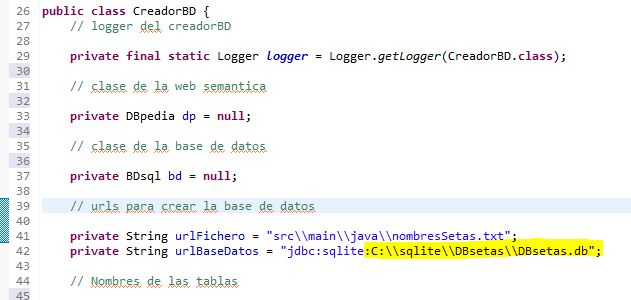
\includegraphics[width=1\textwidth]{imagenesAnexos/imagenesManualProgramador/RutaBaseDatos}%
          \caption{Ruta de la base de datos.}%
          \label{figRutaBaseDatos}%
        \end{center}%
  	\end{center}%
\end{figure}%

Una vez hecho esto, deberemos ejecutar el \textit{main} que encontramos en la clase \textit{src/main/java/dbpedia/DBpedia.java}. El programa realizará las consultas a la \textit{DBpedia} y guardará la información de las especies en la base de datos \textit{SQlite} especificada. Este proceso tardará unos minutos, dependiendo de la velocidad de la conexión a Internet.

La lista de especies de setas a consultar se encuentra en el fichero que encontramos en la ruta \textit{src/main/java/nombresSetas.txt} del proyecto.
Encontraremos la siguiente estructura \ref{figListaEspeciesSetas} en la que podremos añadir o quitar especies para consultar a la DBpedia. 

\begin{figure}[h]
    \begin{center}%
        \begin{center}%
          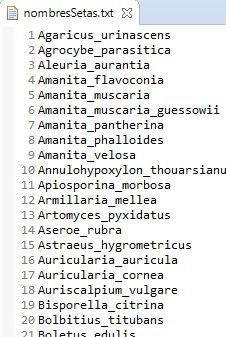
\includegraphics[width=0.5\textwidth]{imagenesAnexos/imagenesManualProgramador/ListaEspeciesSetas}%
          \caption{Listado de especies de setas.}%
          \label{figListaEspeciesSetas}%
        \end{center}%
  	\end{center}%
\end{figure}%

Por último, para instalar la base de datos en la aplicación Android, deberemos copiar nuestro fichero \textit{DBsetas.db} (o el nombre que le hayamos dado) dentro de la carpeta \textit{/app/src/main/assets/databases} del proyecto Android.
\clearpage

\subsection{Extracción de las claves dicotómicas}

En esta sección se explicará como ejecutar el proyecto Eclipse para que extraiga las claves dicotómicas, mediante \textit{web scraping}, de la página web \url{http://www.avelinosetas.info/claves.php}.

Para realizar esta tarea, simplemente deberemos ejecutar el main que se encuentra en la clase \textit{src/main/java/webscraping/ClaveDicotomica.java} del proyecto de Eclipse.

Una vez hayamos ejecutado este programa, se nos habrán creado dos archivos en la raíz del proyecto:
\begin{itemize}
	\item claves.dat: contiene las claves dicotómicas en Español.
	\item clavesEn.dat: contiene las claves dicotómicas en Inglés.
\end{itemize}

Por último, para instalar las claves en la aplicación Android, deberemos copiar nuestros ficheros \textit{claves.dat} y \textit{clavesEn.dat} dentro de la carpeta \textit{/app/src/main/assets/claves} del proyecto Android.

\subsection{Entrenamiento del clasificador}

En este apartado se explicará como usar el proyecto de Tensorflow para entrenar nuestro propio clasificador de imágenes. Este proyecto lo podremos encontrar en la carpeta \textbackslash Herramientas adicionales\textbackslash \textit{image\_retraining}. Tiene la siguiente estructura \ref{figEstructuraImageRetraining}.

\begin{figure}[h]
    \begin{center}%
        \begin{center}%
          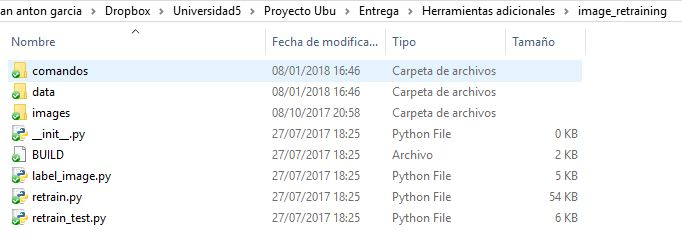
\includegraphics[width=1\textwidth]{imagenesAnexos/imagenesManualProgramador/EstructuraImageRetraining}%
          \caption{Estructura Image Retraining.}%
          \label{figEstructuraImageRetraining}%
        \end{center}%
  	\end{center}%
\end{figure}%

Para hacer uso de este proyecto necesitaremos tener instalados Python y Tensorflow\footnote{\url{https://www.tensorflow.org/install/}} en nuestro sistema.

Lo primero que deberemos hacer es colocar en la carpeta \textit{images} del proyecto nuestras imágenes divididas en carpetas. En cada carpeta colocaremos las imágenes que se correspondan con una misma especie de seta y 
llamaremos a esa carpeta con el nombre de la especie \ref{figListaEspeciesSetas}.

\begin{figure}[h]
    \begin{center}%
        \begin{center}%
          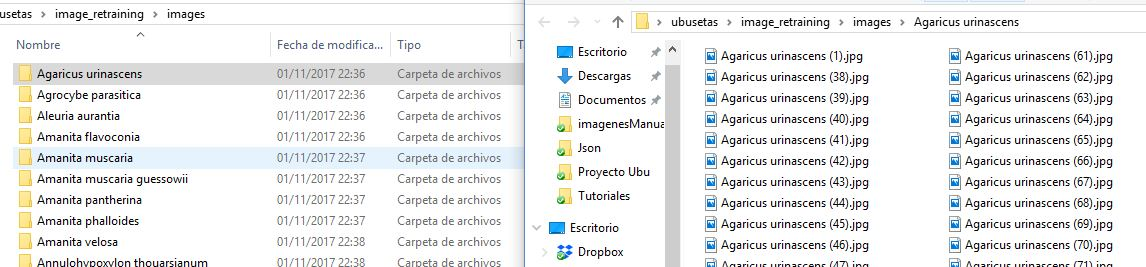
\includegraphics[width=1\textwidth]{imagenesAnexos/imagenesManualProgramador/ListadoEspeciesSetas}%
          \caption{Estructura Image Retraining.}%
          \label{figListadoEspeciesSetas}%
        \end{center}%
  	\end{center}%
\end{figure}%

Si queremos hacer uso del \textit{data augmentation}, deberemos modificar los parámetros dentro del fichero retrain.py, según se indica en las descripciones de estos dentro del código.

Para entrenar el modelo deberemos abrir una consola y colocarnos en la carpeta \textit{image\_retraining}. Una vez aquí deberemos activar Tensorflow con el siguiente comando \ref{figActivacionTensorflow}.

\begin{figure}[h]
    \begin{center}%
        \begin{center}%
          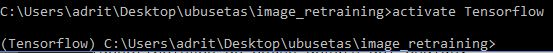
\includegraphics[width=1\textwidth]{imagenesAnexos/imagenesManualProgramador/ActivacionTensorflow}%
          \caption{Activación Tensorflow.}%
          \label{figActivacionTensorflow}%
        \end{center}%
  	\end{center}%
\end{figure}%

Cuando hayamos activado \textit{Tensorflow} podremos ejecutar el fichero retrain.py para entrenar el modelo. Deberemos especificarle el modelo que queremos entrenar, por ejemplo, para entrenar el \textit{Mobilenet-224} ejecutaríamos el siguiente comando \ref{figEntrenamientoTensorflow}.

\begin{figure}[h]
    \begin{center}%
        \begin{center}%
          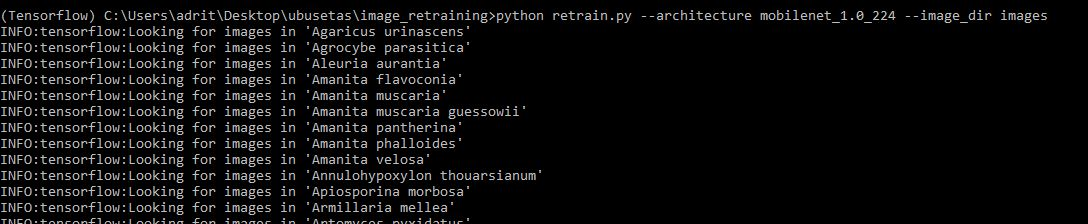
\includegraphics[width=1\textwidth]{imagenesAnexos/imagenesManualProgramador/EntrenamientoTensorflow}%
          \caption{Entrenamiento Mobilenet.}%
          \label{figEntrenamientoTensorflow}%
        \end{center}%
  	\end{center}%
\end{figure}%
\newpage
Cuando el proceso acabe (puede tardar horas o días según la configuración), se nos generarán los siguientes dos archivos en la carpeta C:\textbackslash tmp:

\begin{itemize}
	\item output\_graph.pb: El modelo entrenado.
	\item output\_labels.txt: Los \textit{labels} del modelo.
\end{itemize}

Para instalar nuestro modelo Mobilenet en la aplicación Android deberemos colocar estos dos archivos en la carpeta \textit{/app/src/main/assets/mobilenet-224} del proyecto Android.

\section{Compilación, instalación y ejecución del proyecto}

En esta sección se desarrollarán los pasos necesarios para instalar tanto el proyecto Eclipse como el proyecto Android.

\subsection{Proyecto Eclipse}

En este apartado se explicará como instalar el proyecto de Eclipse llamado \textit{ExtraccionDatos}. Este proyecto lo podemos encontrar en la carpeta \textit{Proyecto Eclipse}, deberemos extraerlo para poder importarlo.

En el proyecto se ha usado la versión de Eclipse Neon.3 Release (4.6.3). Necesitaremos una versión de Eclipse\footnote{\url{http://www.eclipse.org/downloads/eclipse-packages/}} igual o superior a esta para instalarlo. Además necesitaremos tener instalado Maven en Eclipse \footnote{\url{https://maven.apache.org/install.html}}.

Para instalar el proyecto \textit{ExtraccionDatos} deberemos importarlo como un proyecto Maven de la siguiente forma \ref{figImportacionEclipse} \ref{figImportacionEclipse2}.

\begin{figure}[h]
    \begin{center}%
        \begin{center}%
          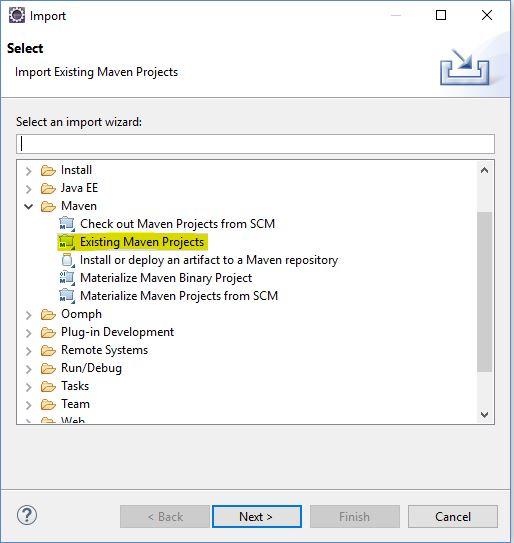
\includegraphics[width=0.6\textwidth]{imagenesAnexos/imagenesManualProgramador/ImportacionEclipse}%
          \caption{Importación Eclipse.}%
          \label{figImportacionEclipse}%
        \end{center}%
  	\end{center}%
\end{figure}%

\begin{figure}[h]
    \begin{center}%
        \begin{center}%
          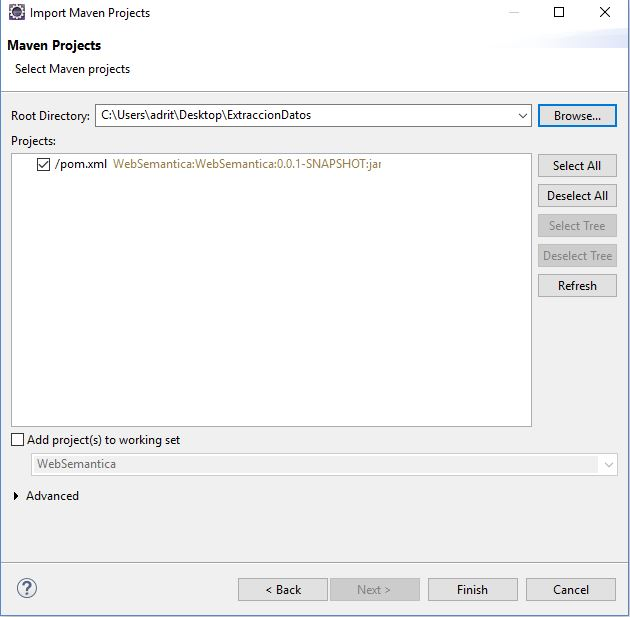
\includegraphics[width=0.6\textwidth]{imagenesAnexos/imagenesManualProgramador/ImportacionEclipse2}%
          \caption{Importación Eclipse.}%
          \label{figImportacionEclipse2}%
        \end{center}%
  	\end{center}%
\end{figure}%

\clearpage
Una vez importado el proyecto base deberemos importar las siguientes librerías al proyecto. Se ha creado un tutorial para cada una que muestra como se descargan e importan al proyecto.

\begin{itemize}
	\item apache-jena-3.4.0: Es la librería que nos proporciona los métodos necesarios para realizar las consultas a la DBpedia. El tutorial se encuentra en el archivo \textit{Tutoriales/Instalación librería Jena en Eclise.pdf}.
	\item jaunt1.3.7: Esta librería nos permite hacer \textit{web scraping}sobre una página Web. Tiene la peculiaridad de que hay que actualizarla cada mes. El tutorial se encuentra en el archivo \textit{Tutoriales/Instalación librería Jaunt en Eclise.pdf}.
	\item json-20171018: Nos permite usar JSON en el proyecto. El tutorial se encuentra en el archivo \textit{Tutoriales/Instalación librería Json.pdf}.
	\item sqlite-jdbc-3.20.0: Nos proporciona los métodos para acceder a la base de datos SQlite. El tutorial se encuentra en el archivo \textit{Tutoriales/Instalación SQlite windows.pdf}.
\end{itemize}

Una vez realizadas las importaciones, ya podremos compilar el programa a través de Eclipse.

\clearpage

\subsection{Proyecto Android}

En este apartado se explicará como se importa el proyecto Android llamado \textit{ProyectoUbusetas}. Este proyecto lo podemos encontrar en la carpeta \textit{Proyecto Android}, deberemos extraerlo para poder importarlo.

Necesitaremos tener instalado en el sistema el entorno de desarrollo Android Studio\footnote{\url{https://developer.android.com/studio/index.html?hl=es-419}}. En este proyecto se ha usado la versión 3.0.1 de Android Studio.

Para importar el proyecto solo habrá que abrir con Android Studio el proyecto proporcionado, automáticamente se descargarán las dependencias necesarias y cuando este proceso acabe, el proyecto estará listo para compilarse.

\subsection{Javadoc}

Tanto el proyecto Android como el Eclipse tienen generados sus correspondientes ficheros Javadoc en los que se ha explicado el funcionamiento de todas las clases y métodos implementados.

\section{Pruebas del sistema}

Las pruebas implementadas se han desarrollado sobre el proyecto Android. Estas pruebas se han dividido en los siguientes 3 tipos:

\begin{itemize}
	\item Pruebas Unitarias \ref{figPruebasUnitarias}: Se han creado pruebas unitarias para probar el correcto funcionamiento de los métodos de las actividades de manera individual. En principio estas pruebas solo cubren el 40\% \ref{figCoverageUnitarias} del código debido a que no puedo probar la mayoría de los elementos de la interfaz con estas pruebas. Estas pruebas se han concentrado en probar los elementos más críticos y que no tienen que ver con la interfaz. Estos códigos no accesibles desde las pruebas unitarias se han probado con las pruebas de integración.
	\item Pruebas de integración \ref{figPruebaIntegracion}: Pruebas que se han creado para comprobar la correcta interacción entre las actividades y el correcto funcionamiento de la interfaz de la aplicación.
	\item Pruebas de rendimiento: Para las pruebas de rendimiento se uso la herramienta \textit{Monkeyrunner}. Esta herramienta se configuró para que ejecutarán 50.000 eventos aleatorios sobre la aplicación y comprobar si se bloqueaba en algún punto. La aplicación consiguió aguantar todos los eventos.
\end{itemize}

La descripción de cada prueba se encuentra en el javadoc del proyecto Android.

\begin{figure}[h]
    \begin{center}%
        \begin{center}%
          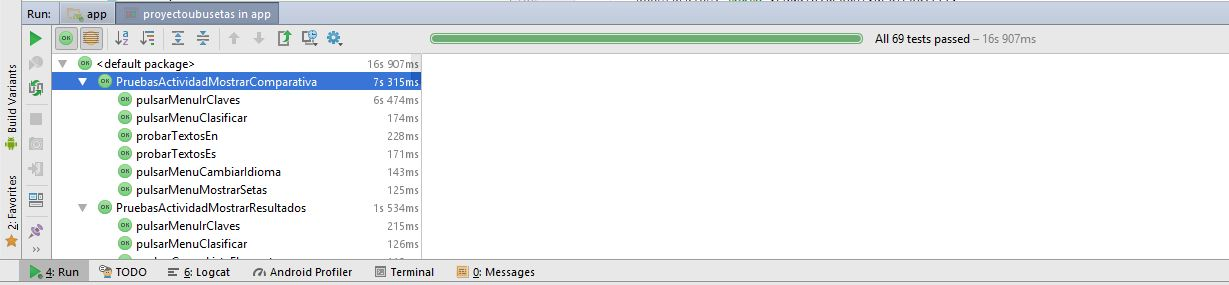
\includegraphics[width=1\textwidth]{imagenesAnexos/imagenesManualProgramador/PruebasUnitarias}%
          \caption{PruebasUnitarias.}%
          \label{figPruebasUnitarias}%
        \end{center}%
  	\end{center}%
\end{figure}%

\begin{figure}[h]
    \begin{center}%
        \begin{center}%
          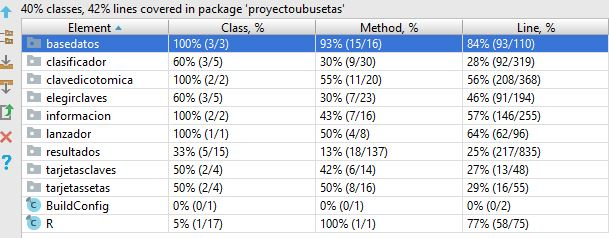
\includegraphics[width=1\textwidth]{imagenesAnexos/imagenesManualProgramador/CoverageUnitarias}%
          \caption{\textit{Coverage} pruebas unitarias.}%
          \label{figCoverageUnitarias}%
        \end{center}%
  	\end{center}%
\end{figure}%

\begin{figure}[h]
    \begin{center}%
        \begin{center}%
          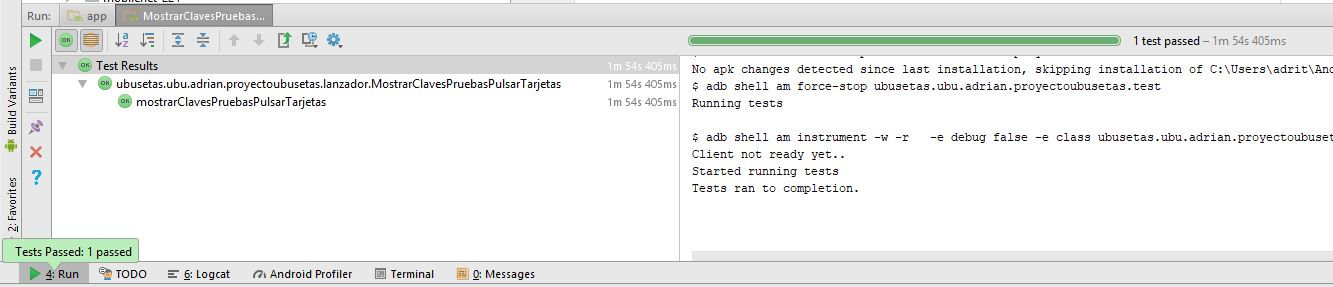
\includegraphics[width=1\textwidth]{imagenesAnexos/imagenesManualProgramador/PruebaIntegracion}%
          \caption{Ejemplo prueba integración.}%
          \label{figPruebaIntegracion}%
        \end{center}%
  	\end{center}%
\end{figure}%